\section{Impact Analysis}
The following impact analysis serves the purpose of analzying stuff TODO: Write more
DESCRIBE THE FEATURE ENDPOINTS USED

\subsection{Featureous Feature-Code Characterization}
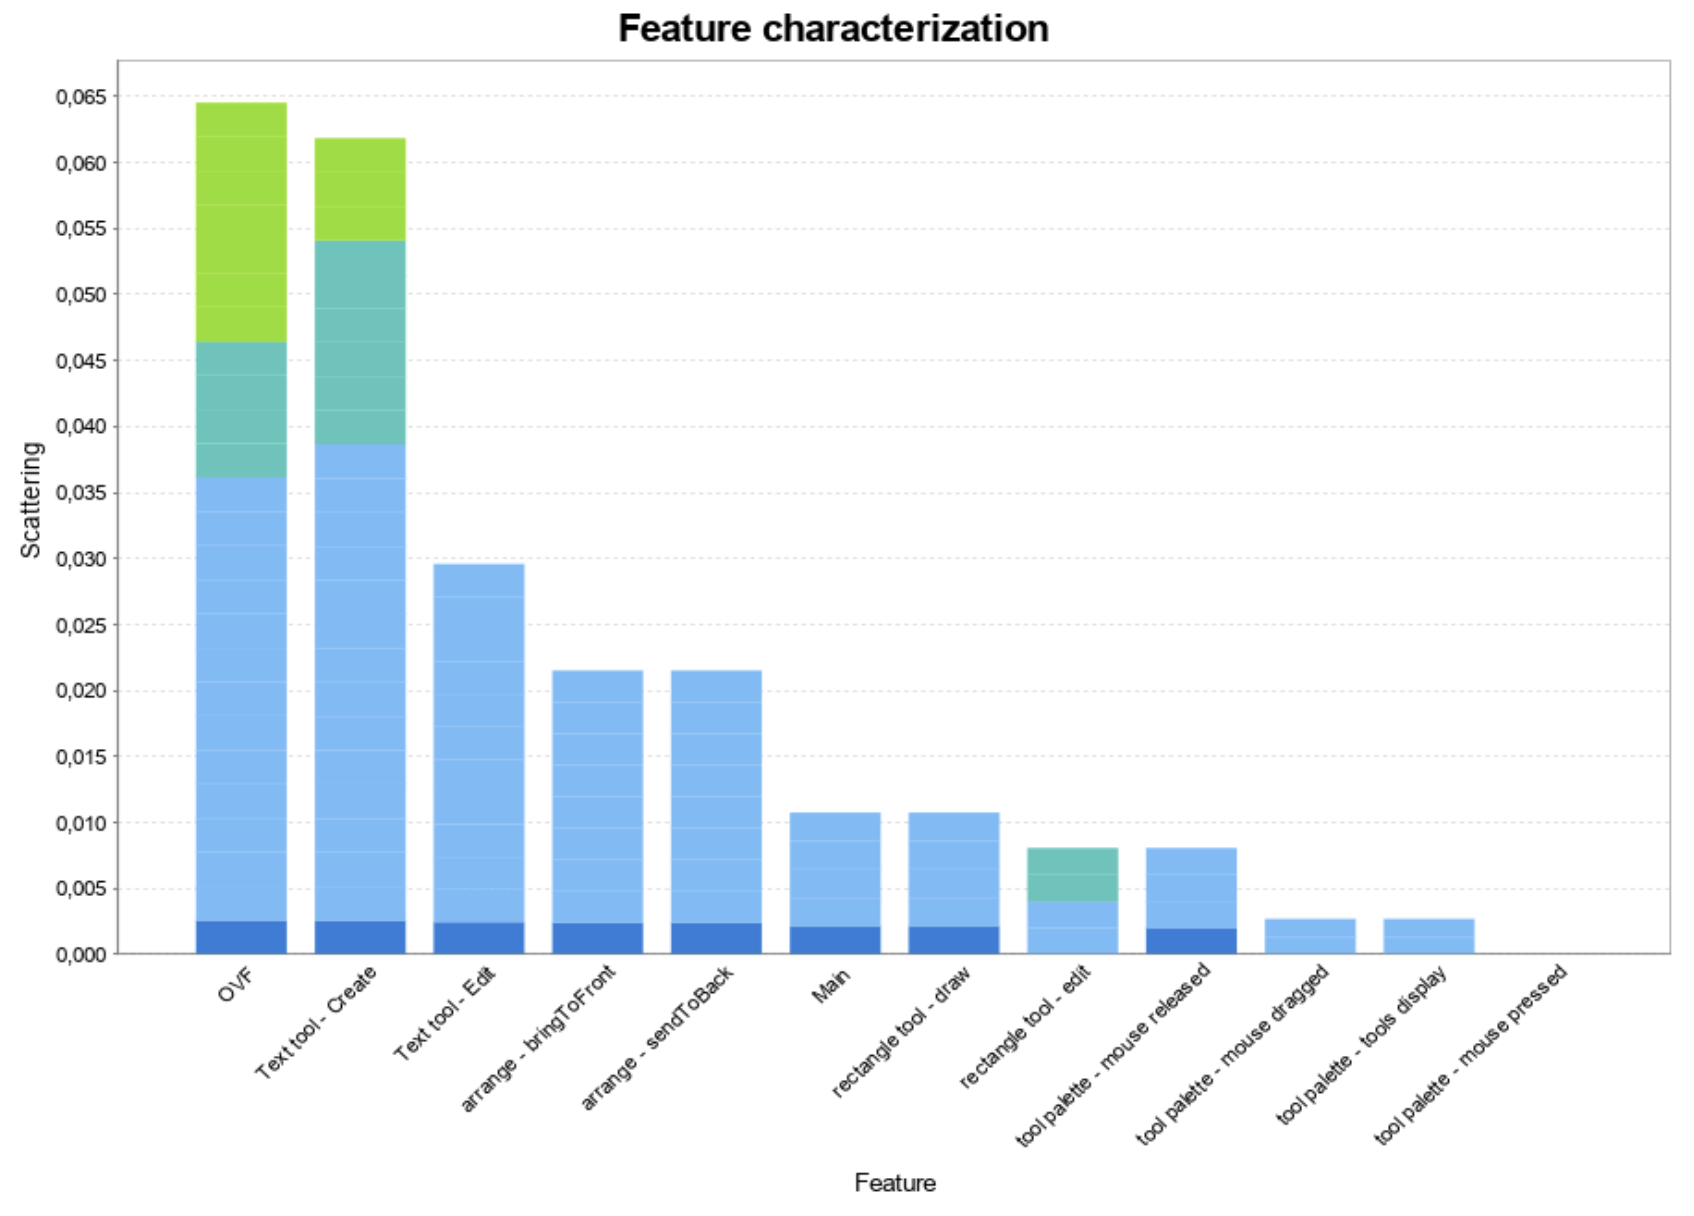
\includegraphics[width=\textwidth]{Images/featurecharacterization.png}
Use Featureous Feature-Code Characterization View to illustrate Scattering and Tangling of each feature that is involved in your Change Request.
Write your reflections about how these measurements relate to your feature and future refactorings. For example, text about the purpose of Impact Analysis and ripple effects.

Use Featureous Feature Relations Characterization view to relate your change request features to each other with respect to how they depend on the objects created by other features and how they exchange data by sharing these objects with one another.

\subsection{Feature Correlation Grid}
\subsection{Feature Correlation Graph}
Use Feature-code correlation graph and feature-code correlation grid to illustrate detailed investigations of the correspondences between source code units and related features to your change request.

Using table 2 list the packages and their number of classes that you visited after you located the concept. Write short comments explaining what you have learned about each package and how they contribute to your feature?
\subsection{Feature Relations Characterization}
\subsection{Dependency Analysis}

Show the features that my feature depends on

\subsection{Impact Analysis}
In the fourth column, mention if the class is related to the concept. Use one of the following terms:
\begin{itemize}
    \item Use “Unchanged” if the class has no relation to the concept but you have visited it.
    \item Use “Propagating” if you read the source code of the class and it guides you to the location of the concept, but you will not change it.
    \item Use “Changed” if the class will be changed.
\end{itemize}


\begin{longtblr}[caption = {The list of all the packages visited during impact analysis.}]{|l|l|l|l|}
    \hline
    \bf{Package name} & \bf{\# of classes} & \bf{Tool used} & \bf{Comments} \\
    \hline
    \bf{}             & \bf{}              & \bf{}          & \bf{}         \\
    \hline
    \bf{}             & \bf{}              & \bf{}          & \bf{}         \\
    \hline
    \bf{}             & \bf{}              & \bf{}          & \bf{}         \\
    \hline
    \bf{}             & \bf{}              & \bf{}          & \bf{}         \\
    \hline
\end{longtblr}
